\documentclass{article}
\usepackage{graphicx}
\usepackage{float}
% if you need to pass options to natbib, use, e.g.:
%     \PassOptionsToPackage{numbers, compress}{natbib}
% before loading neurips_2021

% ready for submission
% \usepackage{neurips_2021}

% to compile a preprint version, e.g., for submission to arXiv, add add the
% [preprint] option:
\usepackage[preprint]{neurips_2021}

% to compile a camera-ready version, add the [final] option, e.g.:
%     \usepackage[final]{neurips_2021}

% to avoid loading the natbib package, add option nonatbib:
%    \usepackage[nonatbib]{neurips_2021}

\usepackage[utf8]{inputenc} % allow utf-8 input
\usepackage[T1]{fontenc}    % use 8-bit T1 fonts
\usepackage{hyperref}       % hyperlinks
\usepackage{url}            % simple URL typesetting
\usepackage{booktabs}       % professional-quality tables
\usepackage{amsfonts}       % blackboard math symbols
\usepackage{nicefrac}       % compact symbols for 1/2, etc.
\usepackage{microtype}      % microtypography
\usepackage{xcolor}         % colors

\title{CSE 151B Project Milestone Report}

% The \author macro works with any number of authors. There are two commands
% used to separate the names and addresses of multiple authors: \And and \AND.
%
% Using \And between authors leaves it to LaTeX to determine where to break the
% lines. Using \AND forces a line break at that point. So, if LaTeX puts 3 of 4
% authors names on the first line, and the last on the second line, try using
% \AND instead of \And before the third author name.

\author{\AND
  Zedian Zhang\\
  \texttt{zez012@ucsd.edu} \\
  \AND
  Christine Nguyen\\
  \texttt{chn012@ucsd.edu} \\
  % examples of more authors
  % \And
  % Coauthor \\
  % Affiliation \\
  % Address \\
  % \texttt{email} \\
  % \AND
  % Coauthor \\
  % Affiliation \\
  % Address \\
  % \texttt{email} \\
  % \And
  % Coauthor \\
  % Affiliation \\
  % Address \\
  % \texttt{email} \\
  % \And
  % Coauthor \\
  % Affiliation \\
  % Address \\
  % \texttt{email} \\
}

\begin{document}

\bibliographystyle{plain}


\maketitle

% \begin{abstract}
%   The abstract paragraph should be indented \nicefrac{1}{2}~inch (3~picas) on
%   both the left- and right-hand margins. Use 10~point type, with a vertical
%   spacing (leading) of 11~points.  The word \textbf{Abstract} must be centered,
%   bold, and in point size 12. Two line spaces precede the abstract. The abstract
%   must be limited to one paragraph.
% \end{abstract}

\section{Task Description and Background}

\subsection{Problem A}

The task of our project is to predict the positions of a tracked object 3 second into the future, given an initial 2-second observation. This is also a regression task since we are dealing with continuous inputs and outputs. It is important because our loss function depends on what task we are dealing with. In our case, since we want to minimize the distance between the prediction and the grand truth, root mean squared error would be the best choice. The ability to plan, conditioned on the future states of dynamic agents in complex roadway environments is a central challenge to the safe and efficient operation of autonomous vehicles. 

This task is important in real world application since progress on the motion prediction problem has downstream consequences for the deployment timeline, scale, and performance of autonomous vehicles as paratransit, long-haul freight, and local delivery options. The most direct application of this in real life is in terms of autonomous vehicles like Tesla's proposed consumer complete self-driving car or autonomous freight vehicles transporting goods, but the  application doesn't have to remain only in terms of autonomous vehicles. For just one example, building on this, we could do prediction of future weather given current weather information. 

\subsection{Problem B}
\textit{Deep Learning-based Vehicle Behavior Predictions for Autonomous Driving Applications: a Review}$^{1}$ outlines multiple approaches to predicting trajectory of an automobile. In the paper, multiple model architectures - include RNNs, CNNs, Graph Neural networks, and various combinations of these - were trained and their test RMSE error was tested over varying second predictions. In general, a Graph Neural Network resulted in the lowest RMSE, but the other architectures still produce a surprisingly close loss. In addition to leveraging multiple architectures, the paper also illustrates the RMSE of these models depending on the type of data input. While most of the models took in an input of both Target Vehicle and Surround Vehicles information, a multi-layer RNN that takes in just the Target Vehicle information performed surprisingly well to that point that if we're only predicting 1 second into the future, it will actually beat out all other models that also track surrounding Vehicle information. \\ \\ 
\textit{Lane-Attention: Predicting Vehicles’ Moving Trajectories by Learning Their Attention Over Lanes}$^{2}$
 proposes the addition of attention to lanes to help model trajectory prediction of automobiles and asserts that it can be done without large cost. An example of this given is using an MLP with LSTM to learn the relative displacement at each timestamp and then use another LSTM network to capture the mathematical projection of vehicles along their lanes to learn a vehicles relation to lanes. We can learn a lane's relative position to a vehicle with another MLP network, and then use a pooling function in order to get the lane closest to the target vehicle. An attention score is then calculated for every lane and used to update the hidden states. This is referred to as the proposed Lane-Attention. Analyzing the result of this model and various other models with and without this Lane-Attention, there is indeed a decrease in Euclidean displacement error when implementing Lane-Attention.

\subsection{Problem C}
The input we are using is a 200 x 1 x 19 x 4 3D matrix. The dimensionality of this input is due to the fact that we use a batch size of 200 with an input of 1 target agent in the scene over 19 timestamps, and 4 because we have 4 features to keep track of: position x, position y, velocity x, and velocity y. The output will be a vector with 60 elements which are the x and y positions of a target agent over 30 timestamps.  

At each timespam in our model, the input is $(x^{t}_{i},y^{t}_{i})$ for $t=\{1,....,T_{obs}\}$ then output is $(x^{t}_{i},y^{t}_{i})$ for $t=\{T_\{obs\},....,T_{pred}\}$ we are predicting one time set each time. This model is mainly use to predicting sequence base on some input sequence, we can potentially use this model to predict stock prices. we can use the past stock price as input to predict future stock prices. Further more, we can use this project to predict sale or warehouse inventory, we can even extend the time step to month or even year for different prediction task. In general, this model could be applied to any time sequenced problem with varying levels of accuracy.
\section{Exploratory Data Analysis}


\subsection{Problem A}
The train data is 205942 pickle file contain information about one scene per file and the test data is 3200 agent vehicle's position and velocity over 19 time step.  \\
The input dimension of the raw data is 60 x 19 x 4 and the output dimension is just 60. The dimensionality of this input is due to the fact that we use an input of 60 possible agents in the scene over 19 timestamps, and 4 because we have 4 features to keep track of: position x, position y, velocity x, and velocity y. The output will be a vector with 60 elements which are the x and y positions of a target agent over 30 timestamps. Figure 1 shows some data samples of the inputs and outputs. 
\begin{figure}[H]
    \centering
    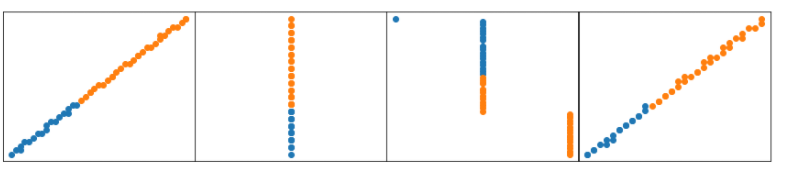
\includegraphics[scale=0.7]{data_smaple.png}
    \caption{4 data samples. The blue being the input trajectory and orange being the ground truth output trajectory.}
    \label{fig:sample_data_points}
\end{figure}
\subsection{Problem B}

\begin{figure}[H]
    \centering
    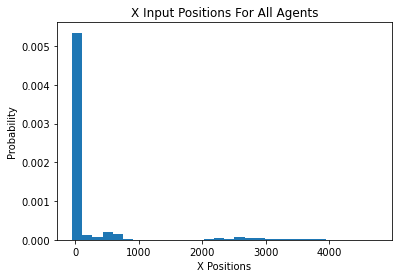
\includegraphics[scale=.5]{p_in_x .png}
    \caption{X Input Positions for All Agents}
    \label{fig:x_input}
\end{figure}
\begin{figure}[H]
    \centering
    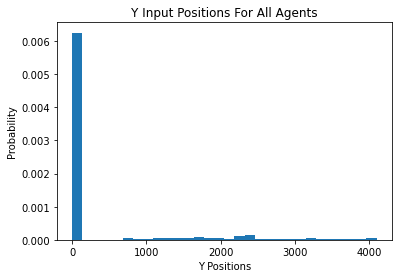
\includegraphics[scale=.5]{p_in_y .png}
    \caption{Y Input Positions for All Agents}
    \label{fig:y_input}
\end{figure}
\begin{figure}[H]
    \centering
    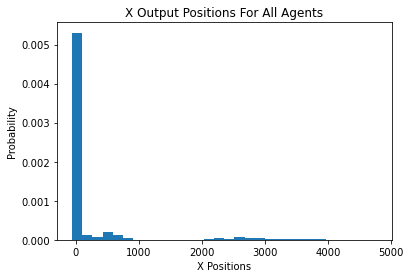
\includegraphics[scale=.5]{p_out_x.png}
    \caption{X Output Positions for All Agents}
    \label{fig:x_output}
\end{figure}
\begin{figure}[H]
    \centering
    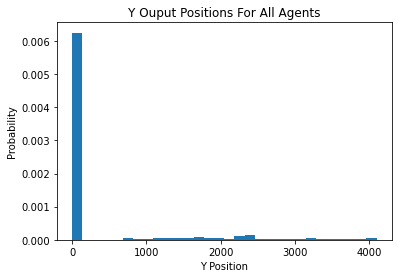
\includegraphics[scale=.5]{p_out_y.png}
    \caption{Y Output Positions for All Agents}
    \label{fig:y_output}
\end{figure}

By looking at Figure 1 and Figure 2, we can see the distribution of input positions for all agents. From the histograms, it seems that the vast majority of input positions for all agents are 0 or very close to 0, with a much smaller number of input positions varying across the range of 0 to 5000. This means that we can safely say that all agent positions will most likely be values close to 0. Table 1 further illustrates this since the mean is a really small number with a standard deviation of 700. 

Figures 1 and 2 show striking similarities with Figure 3 and 4, which implies that input positions and output positions are very similar. This implies that changes in position between input and output are rather small, which in turn implies that input and output velocities should be rather small as well. There is very little difference between the mean of the input and output positions, which further proves that the change in position in scenes are generally very low. 

\begin{table}[H]
  \caption{Input and Output Statistics }
  \label{Training Loss}
  \centering
  \begin{tabular}{rll}
    \toprule
    \cmidrule(r){1-2}
                           & Mean                     & Standard Deviation      \\
    \midrule
    input x position       & 2.16267263e+02           & 716.702954            \\
    input y position       & 3.19052374e+02           & 838.406315            \\
    output x position      & 2.16321698e+02           & 716.823062            \\
    output y position      & 3.18988186e+02           & 838.163668            \\
    all x velocity         & 2.047286016e-02          & 1.67602163            \\
    all y velocity         & -2.38505134e-02          & 2.08297928            \\
    target x velocity      & 0.10567122               & 6.43221111            \\
    target y velocity      & -0.28307088              & 7.80019877            \\
    \bottomrule
  \end{tabular}
\end{table}

\begin{figure}[H]
    \centering
    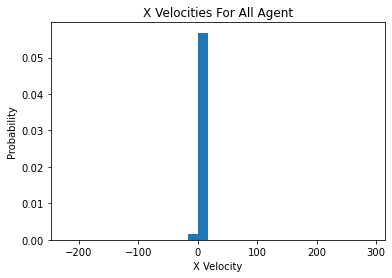
\includegraphics[scale=.5]{v_all_x.png}
    \caption{X Input Velocities for All Agents}
    \label{fig:galaxy}
\end{figure}
\begin{figure}[H]
    \centering
    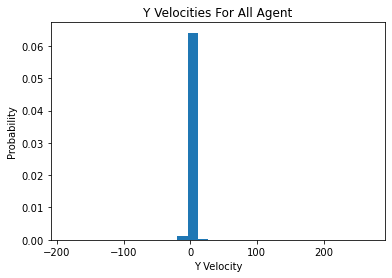
\includegraphics[scale=.5]{v_all_y.png}
    \caption{Y Velocities for All Agents}
    \label{fig:galaxy}
\end{figure}
\begin{figure}[H]
    \centering
    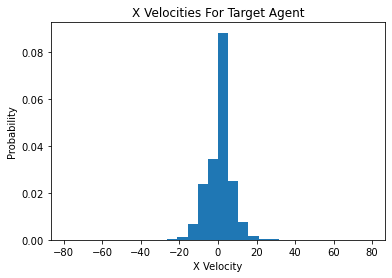
\includegraphics[scale=.5]{v_target_x.png}
    \caption{X Velocities for Target Agents}
    \label{fig:galaxy}
\end{figure}
\begin{figure}[H]
    \centering
    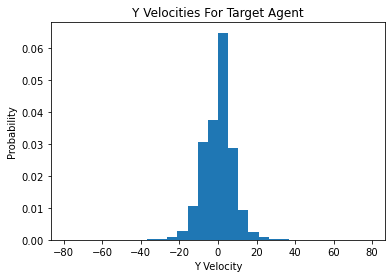
\includegraphics[scale=.5]{v_target_y.png}
    \caption{Y Input Velocities for Target Agents}
    \label{fig:galaxy}
\end{figure}

By looking at Figure 5 and Figure 6, we can see the distribution of velocities for all agents. From the histograms, it seems that the vast majority of input velocities for all agents are 0 or very close to 0. Almost all the velocities can be found in the range of [-30,30]. This is also supported by the standard deviations from Table 1.  This means that we can safely say that overall, agent velocities will most likely be values close to 0. Figures 7 and 8 looks similar to 5 and 6, so this means that target agents velocities don't really deviate from any typical agent's velocities. 

\subsection{Problem C}
The features we chose to use as input to our model is only the target agent's position and velocity of a particular scene. We discarded the data related to other vehicles and the lane information. \\ \\
From here on, we did some feature engineering it that instead of using the position as the input to the model, we instead inputted the change in position paired with the target agent's velocity as the input features. This is also how we normalize the data since the positional features will be in a much smaller range as to emphasize the importance of change in position rather than just position. The reason we chose to use this as normalization is due to the shape of the data. Between every timestamp, vehicles move extremely short distances and their velocities are usually close to 0 as well. This intuitively makes sense since each timestamp is a tenth of a second and not only can vehicles hardly gain any distance in such a short time frame but also most of the vehicles start at a standstill position. Due to this, if we feed in only the position, we'd find the inputs to the model from timestamp to timestamp would be almost identical. This in turn leads to a gradient vanishing problem, so if we emphasize the change in position itself rather than just the position, then we could get a better model. \\ \\
We did not use the lane information provide in the dataset.
\section{Deep Learning Model}
\label{gen_inst}
\subsection{Problem A}
For input we used a batch size of 256 with input features being the velocity and change in position between each timestamp of only the target agent in each scene. The output would be a change in position of the target agent and its velocity for each timestamp. So the shape of the input would be 256 x 19 x 4 and the shape of the output would be 256 x 30 x 4 since we have 19 timestamps in the input and 30 in the output. First we feed 19 timestamps, 1 timestamp at a time into the RNN, which would be a tensor of shape 256 x 4. The output of the encoder at this point will be a vector of 256 hidden features. Now we can predict the following timestamp by inputting the last input timestamp and output hidden features into the decoder. The decoder will then output a vector of 256 x 4, which would represent the predicted next timestamp.\\ \\
The loss function that we ended up using was RMSE since that is the loss that will be used as a final metric of how well our model performs, so it makes sense to minimize this type of loss. Since this is a prediction problem over a continuous value, it doesn't make sense to use other loss functions like Cross Entropy since it's not a categorical problem. \\ \\
We decided on using an encoder-decoder RNN model since the data itself has sequential structure due to the fact that it is tracking a vehicle's position over sequential timestamps. An RNN model would be able to leverage the sequential and temporal spatial structure of the data. Additionally, the input and output are the same in that they both represent the change in position of a vehicle and its velocity, and this output is used as input in the next iteration to predict further timestamps. Naturally this intuitively leads to a RNN model structure since RNN can leverage this similarity. 


\subsection{Problem B}

We tried to use a convolutional neural network in order to make predictions, but faced difficulties trying to propagate through timestamps for multi-step prediction which made it more difficult to design around. \\ \\
Then we switched to an encoder-decoder RNN model, which made designing the model around our task easier since inputs can be fed one by one into the encoder and LSTM hidden states directly rely on the prior hidden state much like with current car position timestamps relying on the previous timestamp.This can then be easily fed into a decoder in much the same manner to predict future timestamps. This is the model that we settled on since it gave us the best results.\\ \\
We tried to add a second LSTM layer to our model, which would essentially double the number of hidden features but that only increased the test loss. Tuning the parameters didn't result in a better test loss, so we did not use this one. 
\\ \\ 
For regularization, we experimented with different dropouts in the encoder and decoder and settled on 0.6 since that resulted in the lowest test RMSE for our model. This helped with the problem of overfitting our model to the data, which resulted in higher test loss. We also reduced the number of data samples we put into the data entirely in order to regularize against overfitting the data. Instead of using the entire dataset for each epoch, we only ever use 15 percent, which resulted in the best loss. At 10 percent of the dataset, the loss increases by around 0.15 and similarly increases at 20 percent. 
\section{Experiment Design}
\subsection{Problem A}

In order to test and train the model, we used the Datahub cloud platform which allows us to leverage a Nvidia 1080 ti gtx gpu for computation. Alongside that, we also used a Nvidia 3070 rtx gpu for testing and training our model computation locally. 

We didn't really split the dataset exactly into training and validation set, since our model only uses 15 percent of the data. Our test loss is based on a separate 15 percent of the data, so that leaves 70 percent of the data untouched entirely. So we have a training set of 15 percent of the provided raw training data and validation set of a differing 15 percent. 

For our optimizer, we used Adam which takes in our weight parameters and a learning rate we set to 0.001. We also tried SGD, RMSProp and  Adadelta with varying learning rates from 0.1 to 0.0001 and found that using the Adam optimizer with learning rate of 0.0001 made the model work best with the least test loss. We also added a learning rate scheduler so that learning rate only updates every 10 steps instead of every step and the update is adding the new learning rate multiplied by gamma of 0.1.  

In order to make the 30 multi-step prediction for each target agent, for the first prediction, we take in a hidden input from the encoder - which would be the change in position from that timestamp and the prior one - and feed that into the decoder, which will give us a prediction of the first timestamp's change in position. By adding that change in position to the previous timestamp, we get the next timestamp's position. Then we recursively feed in the last hidden state from the last timestamp in the decoder in order to get each of the next 29 timestamp positions. Since we are using an encoder-decoder RNN model, making the multi-step prediction in this way is both intuitive and makes the most sense since with car position predictions, previous timestamp positions will directly affect the current timestamp position. 

Running the model with an epoch of 1200 and batch size of 250 gave the best result so far. One epoch takes 10 seconds to run - this is because we're using only a small part of the training data and only use the target agent's position and velocity. Less and more epochs don't perform as well on test data. Changing the batch size either worsen the test loss or have no significant effect on it and we can't try a really big batch size such as the entire data set in a batch due to lack of memory capacity on our utilized GPU. 

\section{Experiment Results}
\subsection{Problem A}

\begin{table}[H]
  \caption{Model comparison}
  \label{model comparsion}
  \centering
  \begin{tabular}{lll}
    \toprule
    \cmidrule(r){1-2}
     & Single layer    & multi-layer (2 layer)    \\
    \midrule
    Epoch    &  40      &  200      \\
    Learning rate        &     0.001     &  0.001     \\
    Batch size &        256        &          256 \\
    Optimizer&  Adam with scheduler & Adam with scheduler\\
    data set size & 15\%              & 15\%    \\
    \# of parameters &  21005316 &         29402116  \\
    time for one epoch &    30 second            & 20 second \\
    \bottomrule
  \end{tabular}
\end{table}
Table 2 show hyper-parameter of two models, they are all encoder decoder LSTM model, the main difference is one is single layer of LSTM cell and the other one is two layer of LSTM cell.


\begin{center}
    Single layer training loss and testing loss 
    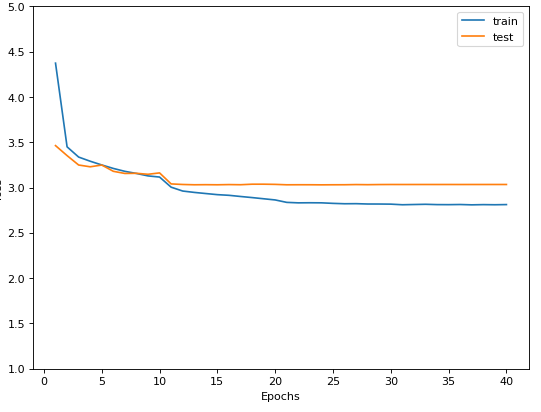
\includegraphics[scale=0.7]{single_loss.png}
\end{center}

\begin{center}
    multi-layer training loss and testing loss 
    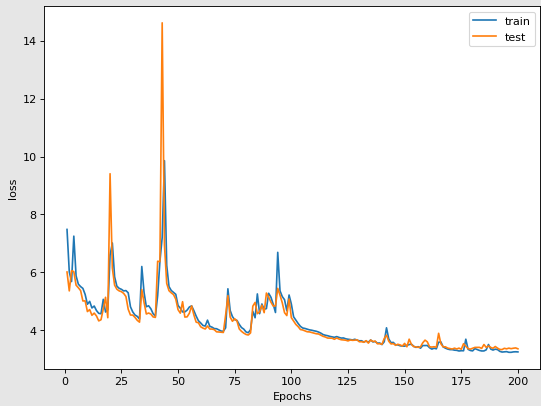
\includegraphics[scale=0.7]{mutil_loss.png}
\end{center}
By looking at the plot, the performance of two model are the same, however the multi-layer model takes more epoch to converge, and the multi-layer model takes longer to train, and have probability of over fitting. One big improvement we did to reduce the training time is we cut down the data set size for training. if we use the whole 20k data set, it takes 10 min to train for one epoch, also we are facing high probability of over fitting. 
\subsection{Problem B}
\begin{center}
    Single layer training loss and testing loss 
    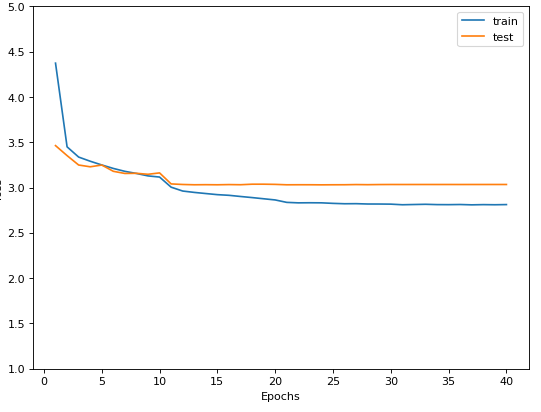
\includegraphics[scale=0.7]{single_loss.png}\\
    training/validation loss (RMSE) value over 40 steps
\end{center}
Our best-performing model is single layer encoder decode LSTM model, follow closely with following structure:
\begin{center}
    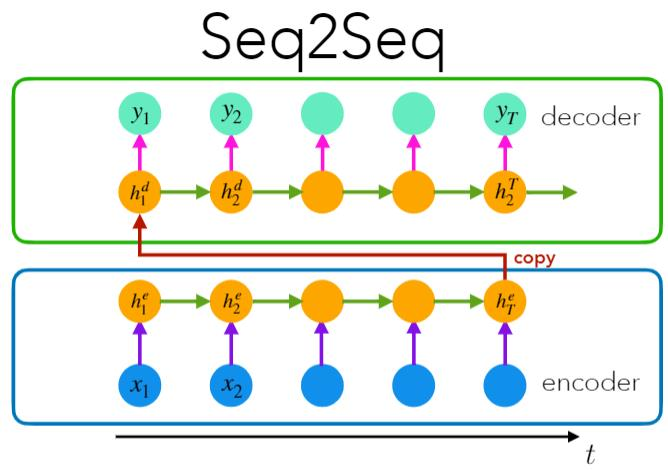
\includegraphics[scale=0.7]{model.jpg}
\end{center}
we discard the outputs in the encoder and only keep the hidden state, feed decoder with the hidden state form encoder and use the model's own prediction from precious step as input.\\

\begin{figure}[H]
    \centering
    This figure shows 12 different training samples with the input, ground truth, and predictions graphed and labeled. 
    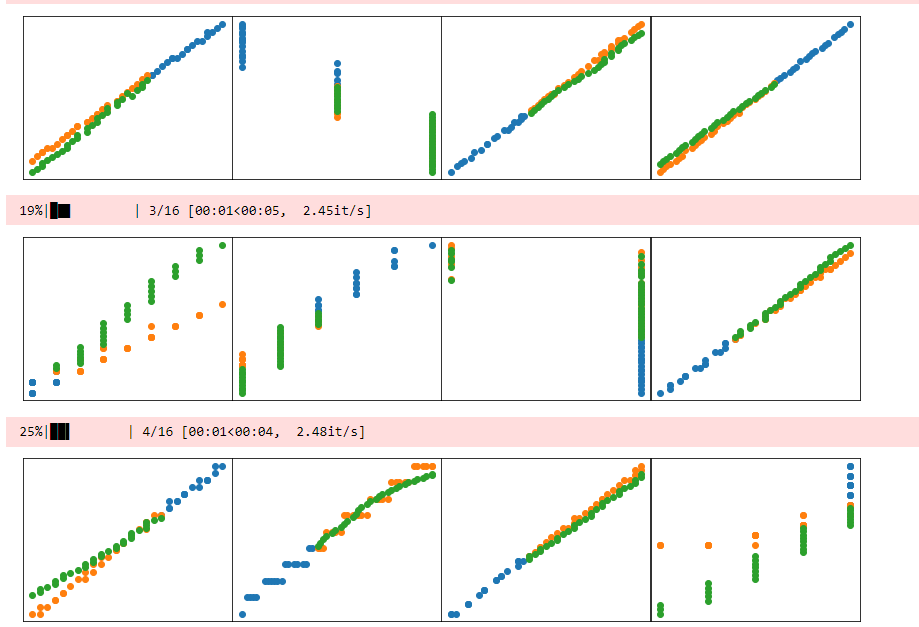
\includegraphics[scale=0.4]{sample.png}
    \caption{12 Training Samples with input (blue), ground truth (orange) and prediction (green)}
    \label{fig:galaxy}
\end{figure}


We are 10th top team with public test RMSE of 2.25084 and private test RMSE of 2.38143.

\section{Discussion and Future Work}
\subsection{Problem A}
We found the most effective feature engineering strategy is to first do a substantial amount of data visualization before choosing your features or even creating a model. Without knowing what your data looks like, it's easy to end up choosing features that increases noise and make your data worse. You could also end up putting more data into your model than you need, which would then result in your model taking much longer to run than is necessary, so you'd waste time on just training your model instead of improving your model. Sometimes less data is better. 

The two techniques that we found to be the most helpful in improving score was data visualization and hyper-parameter tuning. For a long time, even though we were tuning our parameters, our loss was stuck at around 200 because we had not done any data visualization beyond just checking the shape and meaning of the data. As such, we kept our inputs as just target position and velocity. It wasn't until we printed out a bunch of the data points and did an analysis of the distribution that we realize that the inputs positions are actually very close to each other from scene to scene was well as timestamp to timestamp. Knowing this, we were able to feature engineer using change in position of the target agent as input instead of just position. This also prompted us to use a smaller subset of the data for faster learning and reducing overfitting. From there, hyper-parameter tuning of the model made our model jump down to a test RMSE of 2.25084, so I would say that's the second most important technique in improving score. Changing parameters like epoch number, learning rate, learning scheduler parameters, number of hidden features, and batch size went a long way to helping improve our model every time. 

The biggest bottleneck for us in this project was likely training time. Since we are using an LSTM encoder-decoder RNN structure with large number of hidden features, when we were training over the entire dataset, one epoch could take 10 minutes. Another thing that contributed to each epoch taking so long was the fact that if we were running the notebook locally on a Windows device, you could not change the number of workers parameter in the data loader, so the data loader iterating through each batch took an immense amount of time itself without even accounting for training. 

If we were to advise a deep learning beginner how to design deep learning models for similar prediction takes, we'd say that the first thing that they should do is to data visualization. Before designing any model or engineering any features, it would be so helpful to see what the data looks like and what their distribution is so that you can better design your model and features. We were stuck at a loss of 200 for a long time because we chose the wrong input feature since we had not done any data visualization, so we wasted a lot of time. After that, the next biggest advise we can give is to be patient. As we saw during the top 10 presentations, many models can do this prediction task well, but regardless of the model tuning hyper-parameters for a model is very important and will be the most time consuming part of the task. Training over large data sets take a long time, and this time only increases with each epoch, so tuning hyper-parameters will take a long time. It's important to just be patient as you do this. 

If we had other resources, we'd like to try how to implement this as a Graph Neural Network. From the papers we listed earlier, Graph Neural Networks seem to perform the best on automobile trajectory prediction and in lecture we learned that right now it is one of the leading fields of research and development in deep learning, so it would be really interesting to try to create a Graph Neural Network and train it to do this prediction task. 
\section{GitHub Repository}
https://github.com/chn012/cse151b-project

\begin{thebibliography}{9}
\bibitem{autoReview} 
Sajjad Mozaffari, Omar Y. Al-Jarrah, Mehrdad Dianati, Paul Jennings, and Alexandros Mouzakitis 
\textit{Deep Learning-based Vehicle Behaviour Prediction for Autonomous Driving Applications: a Review}
\\\texttt{https://arxiv.org/pdf/1912.11676.pdf}

\bibitem{knuthwebsite} 
Jiacheng Pan, Hongyi Sun, Kecheng Xu, Yifei Jiang1, Xiangquan Xiao, Jiangtao Hu1, and Jinghao Miao
\textit{Lane-Attention: Predicting Vehicles’ Moving Trajectories by Learning Their Attention Over Lanes}
\\\texttt{http://ras.papercept.net/images/temp/IROS/files/1313.pdf}
\end{thebibliography}
\end{document}